\chapter{Introdução}

As metodologias ágeis vem ganhando cada vez espaço no mercado global 
de desenvolvimento de software, pois enfatizam a qualidade do produto 
sobre a qualidade do processo, procurando minimizar a execução 
de atividades não essenciais ao longo do ciclo de vida de 
desenvolvimento de software. 

O eXtreme Programming (XP), que é uma metodologia ágil, tem a codificação como a 
atividade chave durante um projeto de desenvolvimento de software 
\cite{beck1999}. Isso se torna perceptível quando se analisa algumas práticas do 
XP,~\footnote{Documentação disponível em \url{http://www.extremeprogramming.org}}
tais como:

\begin{enumerate}
%-----------------------------
\item Padronização do Código: O código é a principal forma de comunicação entre 
a equipe, logo a padronização de código o torna consistente e fácil para todo o 
time ler e refatorar. 
%-----------------------------
\item Propriedade Coletiva do Código: Cada programador pode melhorar qualquer 
parte do código quando existir a oportunidade.
%-----------------------------
\item Programação em Pares: Todo código é escrito com duas pessoas: uma que olha 
para uma máquina, e outra com um teclado e um mouse.
%-----------------------------
\item Integração Contínua: Todo novo código é integrado ao sistema e quando 
integrado, o sistema é totalmente reconstruído do zero e todos os testes devem 
passar ou o novo código é descartado.

\end{enumerate} 

Dado a importância do código-fonte, infere-se a qualidade do trabalho produzido, 
pela qualidade do código-fonte, sendo que um dos métodos mais utilizados
para tal é a análise estática de código. 

Durante anos, vários trabalhos foram publicados visando a definição formal de 
métodos de análise estática de código-fonte. Vide os trabalhos de 
\citeonline{Wichmann95}, \citeonline{Nielson:1999}, \citeonline{Emanuelsson2008}.
Contudo as ferramentas que realizam o procedimento no código-fonte ainda 
apresentam problemas, tais como:

\newlist{problems}{enumerate}{4}
\setlist[problems]{ label* = P\arabic* -}

\begin{problems}
    \item Ausência de resultados consolidados do produto, pois a maior 
	parte das métricas é extraída de elementos internos menores (Bibliotecas, 
	Pacotes, Classes,Métodos, Funções) do código-fonte.
    
	\item Ausência de mecanismos de tratamento, separação, recuperação e 
	organização e persistência de dados. 
	
	\item Ausência de associação entre resultados numéricos e forma de 
	interpretá-los: Ferramentas de análise estática frequentemente mostram 
	seus resultados como valores numéricos isolados para cada métrica 
	\cite{Meirelles2013}. 
	
	\item Em grande parte das ferramentas, a visualização dos resultados não é 
	agradável, isto é, são apresentados um conjunto de dados em uma janela 
	terminal contendo os valores das métricas.
	
    \end{problems}
	
Os problemas enunciados acima trazem muitos prejuízos à organizações que 
utilizam processos de aferição de qualidade de código-fonte como um indicador do
desenvolvimento de produtos de software, pois sem possibilidade de manter 
registros das métricas de código-fonte, torna-se inviável qualquer análise 
temporal da evolução da qualidade do código-fonte e além disso, se os dados não 
são representativos, qualquer análise fica a cargo de experiências anteriores 
com as métricas de código-fonte.

Dado este contexto, é crucial que dados relacionados a métricas sejam coletados 
e compartilhados entre projetos e pessoas, em uma visão organizacional, 
para que determinada organização ou time possa compreender o processo de medição 
e monitoramento de projetos de software e, consequentemente, se 
tornar mais hábil e eficiente em realizar atividades técnicas relacionadas ao 
processo de desenvolvimento de software 
\cite{Chulani2003}.

Vários trabalhos tem mostrado que ambientes de DWing são boas soluções para 
atender a visão organizacional unificada de métricas de software proposta por 
\citeonline{Chulani2003}. Vide os trabalhos de \citeonline{Palza2003}, 
\citeonline{Ruiz2005}, \citeonline{Castellanos2005}, \citeonline{Becker2006}, 
\citeonline{Folleco2007}, \citeonline{Silveira2010}.


Tendo os trabalhos, enunciados anteriormente, como norteadores, adotou-se como 
hipótese de pesquisa deste trabalho que a \textbf{visualização
e a extração de métricas de código-fonte em ambientes de DWing supre os problemas
encontrados nas ferramentas de análise estática de código-fonte}.


%------------------------------------------------------------------------------%





%------------------------------------------------------------------------------%

\section{Objetivos}

Esta seção apresenta os objetivos gerais e específicos deste TCC.

\subsection{Objetivos Gerais}
Sob prisma da hipótese de pesquisa, há como objetivo geral a proposição e 
construção um ambiente de \textit{Dwing}, para extrair e visualizar métricas de
código-fonte.


%------------------------------------------------------------------------------%

\subsection{Objetivos Específicos}

Os objetivos específicos desse trabalho são:

\newlist{objectives}{enumerate}{3}
\setlist[objectives]{ label* = OE\arabic* -}

\begin{objectives}
	\item Construir o ambiente de Dwing para extração e visualização de métricas 
	de código-fonte utilizando ferramentas de software livre.
  
	\item Incorporar indicadores qualitativos para cada métrica de código-fonte.
	
	\item Facilitar o entendimento das métricas de código-fonte.
	
	\item Apresentar em formas visuais, as análises obtidas das métricas de 
	código-fonte.
	
    \end{objectives}
	


%------------------------------------------------------------------------------%

\section{Sobre o Trabalho}
%------------------------------------------------------------------------------%
\subsection {Metodologia de Pesquisa}
A metodologia de pesquisa foi definida em \textbf{aplicada}, pois visa construir 
conhecimento, em aplicações práticas, dirigido á solução de problemas 
específicos \cite{Gil2008}; \textbf{pesquisa-ação}



\subsection{Cronograma}
O Trabalho de Conclusão de Curso foi planejado, em longo prazo,em quatro ciclos 
de desenvolvimento de vinte e um dias cada um. 
As figuras \ref{cronograma} e \ref{gantt}, que foram extraídas da ferramenta 
OpenProj\footnote{Documentação e \textit{download} disponível em 
\url{http://sourceforge.net/projects/openproj/}}, 
apresentam o cronograma geral o gráfico de Gantt do presente trabalho.

\begin{figure}[h]
\centering
	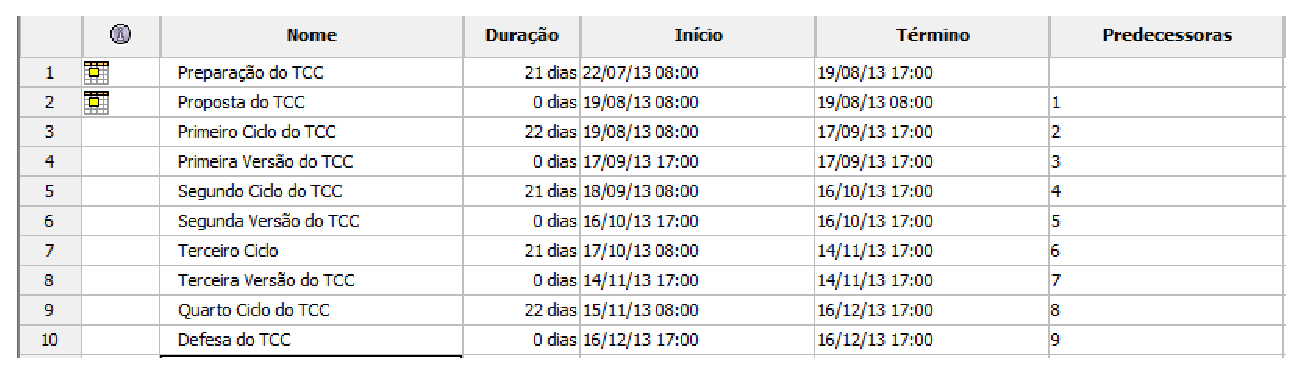
\includegraphics[keepaspectratio=true,scale=0.7]{figuras/marcos.eps}
	\caption{Ciclos de Desenvolvimento do Trabalho de Conclusão de Curso}
	\label{cronograma}
\end{figure}

\clearpage

\begin{figure}[h]
\centering
	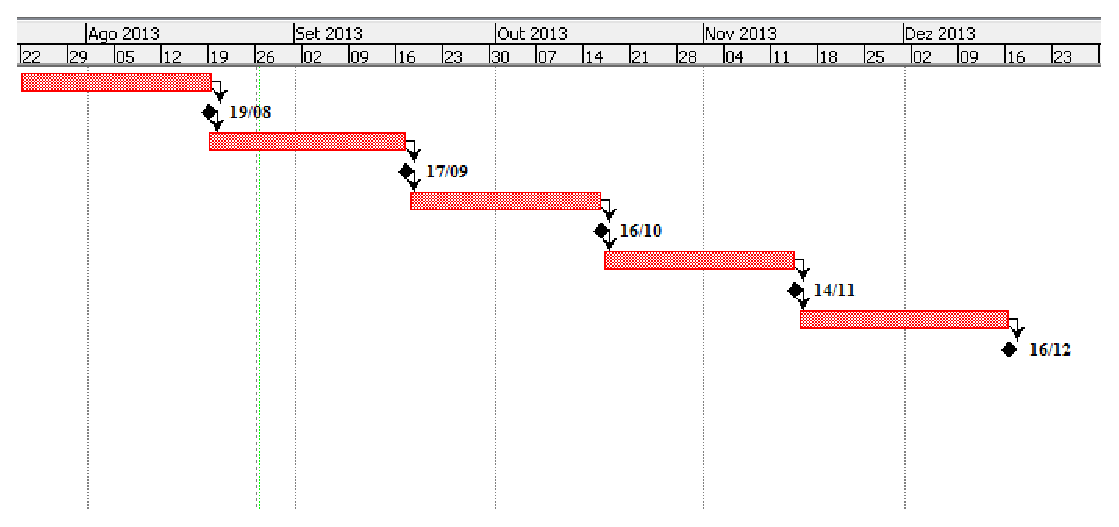
\includegraphics[keepaspectratio=true,scale=0.7]{figuras/gantt_chart.eps}
	\caption{Gráfico de Gantt do Trabalho de Conclusão de Curso}
	\label{gantt}
\end{figure}

Para cada ciclo de desenvolvimento do Trabalho de Conclusão de Curso,  
utilizou-se o Quadro \textit{Kanban} para controle das atividades. 
O termo \textit{kanban} vem do japonês e significa literalmente "cartão". 
O quadro \textit{kanban}, surgiu na Toyota, como um meio visual para controlar o 
fluxo da produção, limitando o tamanho do trabalho em progresso 
\cite{moura1999kanban}.

Posteriormente, o método foi incorporado no processo de desenvolvimento de 
software na  pela metodologia ágil, \textit{Scrum} \cite{Schwaber:2004}. 
O quadro \textit{Kanban} 
que foi utilizado no presente trabalho, foi criado na ferramenta \textit{online}, 
\textit{Kanban Flow},\footnote{Disponível em \url{https://kanbanflow.com}} e foi
 dividido em três colunas: \textbf{Backlog}, que são tarefas a fazer, 
\textbf{Em Progresso}, que são tarefas iniciadas e \textbf{Concluído} que mostra
 as tarefas que já foram executadas. A figura \ref{kanban} mostra o 
 \textit{Kanban} ao final do segundo ciclo de 
desenvolvimento.

\begin{figure}[h]
\centering
	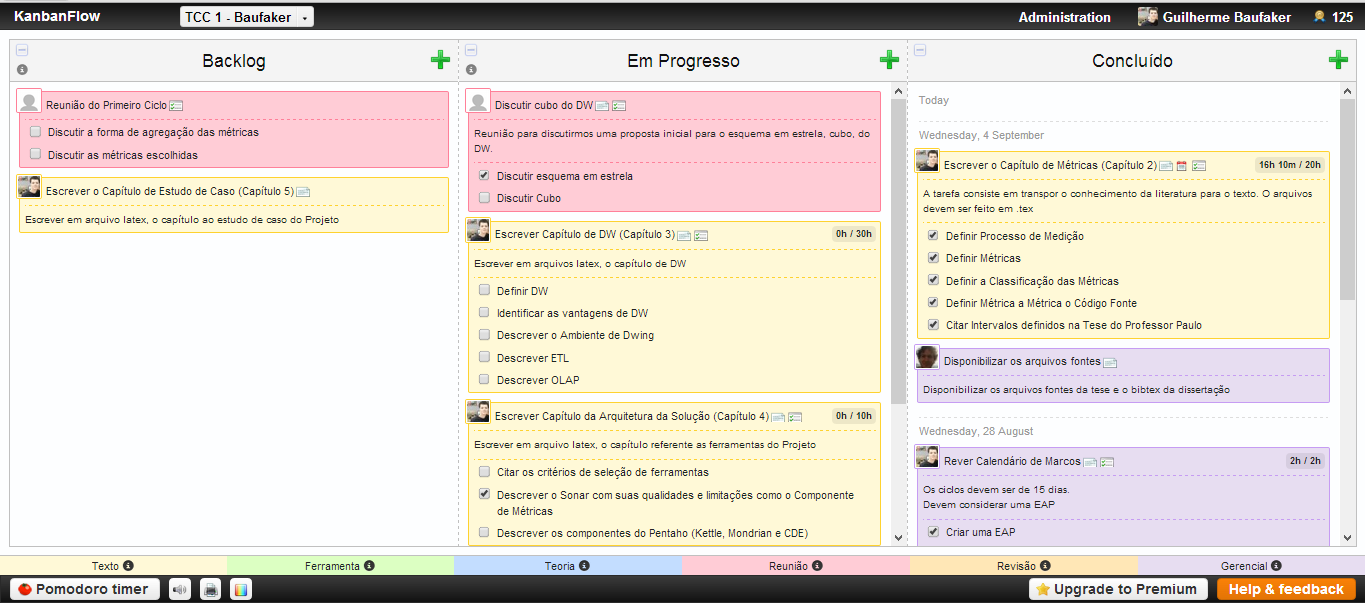
\includegraphics[keepaspectratio=true,scale=0.40]{figuras/kanban.eps}
	\caption{Quadro \textit{Kanban} do Trabalho de Conclusão de Curso}
	\label{kanban}
\end{figure}

Todas as tarefas necessárias para realização deste trabalho de conclusão de 
curso foram listadas no apêndice \ref{kanban flow}. 


\subsection{Organização do Trabalho}
Para a primeira fase deste Trabalho de Conclusão de Curso, além desta introdução 
este texto está organizado em capítulos. O Capítulo 2 apresenta  o processo de 
medição e as métricas de código-fonte.
O Capítulo 3 apresenta o SonarQube como a ferramenta escolhida para extração das 
métricas de código-fonte.
O Capítulo 4 apresenta a fundamentação teórica do ambiente de Dwing, de modo a 
suprir as limitações das ferramentas, e cada um de seus componentes em detalhes. 
O Capítulo 5 apresenta o ambiente proposto por este trabalho para extração e 
visualização das métricas de código-fonte. Por fim, o Capítulo 6 apresenta o 
estado atual da validação 
do ambiente por meio de estudo de caso, bem como as atividades planejadas até o 
encerramento do trabalho de conclusão de curso.
